%-------------------------------------------------------------------
% This is a template for IRAM Proposals (originally created by R.Lucas)
% Deadline 12 Sep 2013
% Please use always the most recent update of proposal.sty
% (R. Neri / C.Thum / J.M.Winters (11 Jul 2013)
% 
%-------------------------------------------------------------------
% ATTENTION:
%
% The following lines follow the LaTeX2e syntax.
%
\documentclass[12pt,a4]{article}
\usepackage{proposal}
\usepackage{graphicx}
%-------------------------------------------------------------------
\begin{document}
%-------------------------------------------------------------------
% Instrument (%sign  comment in or out)
%-------------------------------------------------------------------
\picoveleta
%\blank
%-------------------------------------------------------------------
% Title (replace content)
%-------------------------------------------------------------------
\title{NIKA polarization 2014 October run}
%-------------------------------------------------------------------
% Proposal Type (%sign  comment in or out)
%-------------------------------------------------------------------
%\exgalcont
%\exgalco
\exgalother
%\solarcont
%\solarlines
\solarother
%\galcont
%\gallines
%\galcloud
%\galcse
%\galyse
%\galchem
\galother
%-------------------------------------------------------------------
% Abstract (replace content)
%-------------------------------------------------------------------
\abstract{This is an internal IRAM document to plan the next NIKA polarization
  2014 October technical run to be performed between 4 and 14 October 2014. We
  request 56 hours of observational time to test the NIKA polarization
  capabilities with a new multi-layers HWP and an additional optical element
  (Wollaston prism). In addition we plan to observed 9 astrophysical sources
  (3 extended sources and 6 point sources) with a noise level for the degree
  of polarization of about 1~\%. Two accompanying sessions using XPOL are
  requested, to be adjacent to this NIKA polarization session in order to
  cross-calibrate the two experiments in terms of the polarization angle and
  the degree of polarization.  }
%-------------------------------------------------------------------
% Proposal history : fill in or comment out
%
% If this proposal is a continuation or a resubmission of a previous
% IRAM proposal, please describe the history of the proposal using
% the \proposalhistory{} command at the end of this file. 
%
%-------------------------------------------------------------------
%\resubmit{000-86}
%\continue{000-86}
%-------------------------------------------------------------------
% Amount of telescope time 
%-------------------------------------------------------------------
% Total telescope time requested for this  semester
\hours{64}			
% telescope time, hours, requested 
% NOTE: telescope time includes all overheads, like in the Time Estimator
%-------------------------------------------------------------------
% Receivers (remove the '%' sign when using the receiver) 
% argument: telescope time, hours, requested for this receiver 
%-------------------------------------------------------------------
\emir{8}
%\hera{2.7}
%\gismo{3.8}
\nika{56}
%-------------------------------------------------------------------
% Sidereal time intervals: {start hour}{end hour}{number of intervals} 
%-------------------------------------------------------------------
%\lsta{11}{11}{10}
%\lstb{23}{23}{10}
%----------------------------------------------------------------
% Special requirements 
%----------------------------------------------------------------
%\LargeProgram
%\pooledobserving
%\serviceobserving
%\remoteobserving
\polarimeter
%----------------------------------------------------------------
% Scheduling constraints
%----------------------------------------------------------------
\constraints{None}
%----------------------------------------------------------------
% Principal Investigator (name, institut, address, telephone, email)
%----------------------------------------------------------------
\pifirstname{Andrea Catalano \&}
\pilastname{Nicolas Ponthieu}
\piinstitute{LPSC/IPAG - Grenoble}
\pistreetandnumber{53, rue des Martyrs}
\pizipandcity{38026 Orsay}
\picountry{France}
\piphone{(+33) 4 76 28 41 52 }
\pifax{(+33) 4 76 28 40 04}
\piemail{catalano@lpsc.in2p3.fr \& Nicolas.Ponthieu@obs.ujf-grenoble.fr}
%----------------------------------------------------------------
% A brief remark in case the proposed observations are part 
% of a Diploma thesis, PhD thesis, Marie-Curie fellowship, ... 
% specify here who is the fellow, who the supervisor, ... 
%----------------------------------------------------------------
%\pinote{}      
%----------------------------------------------------------------
% Coauthors 
% macro: \coauthor{First_Name Last_Name}{affiliation}{country} 
% use one \coauthor{ }{ }{ } macro for each coauthor. 
\coauthor{Clemens Thum}{IRAM Granada}{Spain}
\coauthor{Helmut Wiesemeyer}{MPIfR Bonn}{Germany}
\coauthor{Alessia Ritacco}{LPSC Grenoble}{France}
\coauthor{Alain Benoit}{IN Grenoble}{France}
\coauthor{Albrecht Sievers}{IRAM Granada}{Spain}
\coauthor{Vincent Reveret}{CEA Saclay}{France}
% You may add as many \coauthor{ }{ }{ } macros as needed ...
%----------------------------------------------------------------
%\coauthor{Muhammad ibn Musa al-Khwarizmi}{House of Wisdom}{Bagdad}
%\coauthor{Gustav Robert Kirchhoff}{Ruprecht-Karls-Universit\"at Heidelberg}{Germany}
%\coauthor{Charles Messier}{Observatoire de l'H\^{o}tel de Cluny, Paris}{France}
%\coauthor{Jules Janssen}{Observatoire de Paris-Meudon}{France}
%\coauthor{NIKA Core Team see http://ipag.osug.fr/nika2/Collaborators.html}
% ...
%----------------------------------------------------------------
\observer{Catalano, Ponthieu, Ritacco, Benoit}{}{}                 
%----------------------------------------------------------------
% Source list
% One line for each source should be given:
%
% Name   & RA      &    DEC    &   V(LSR) or z(radio) \\
% The epoch is given as a separate parameter.
% ADDITIONAL souces which do not fit here shall be entered in
% the macro "\extendedsourcelist" listed at the end of this file
%----------------------------------------------------------------
\epoch{J2000.0}  % J2000 epoch coordinates preferred
\sourcelist{
Venus &  & & \\
Uranus &  & & \\
Mars &  & & \\
Crab     & 05:34:31.950   & +22:00:52.1  &\\
CasA     & 23:23:27.850   & +58:48:42.8  &\\
KL       & 05:35:14.500   & -05:22:30.0  &\\
DR21\_OH & 20:39:01.100   & +42:22:50.2  &\\
3C84     & 03:19:48.154   & +41:30:42.1  & 6   Jy@1mm, 5.3\% \\
3C286    & 13:31:08.300   & +30:30:33.0  & 0.3 Jy, 14.4\% Pol. Ref. quasar\\
3C345    & 16:42:58.800   & +39:48:37.0  & 2.6 Jy, 7.1\% \\       
1921-293 & 19:24:51.056   & -29:14:30.1  & 6.2 Jy, 7.8\% =OV-236\\
2200+420 & 22:02:43.291   & +42:16:39.9  & 5.5 Jy, 12\% =BL LAC\\
}

%----------------------------------------------------------------
% The following command will actually produce the front page. 
%----------------------------------------------------------------
\frontpage
%
%================================================================
%-NEW--30M--NEW--30M--NEW--30M--NEW--30m--NEW--30M--NEW--30M--NEW
%
%-30M--NEW--30M--NEW--30M--NEW--30M--NEW--30M--NEW--30M--NEW--30M
%----------------------------------------------------------------
%
%--- EMIR -------- EMIR -------- EMIR
%
%enter up to 2 \EMIR parameters macros for each setup 
%each macro MUST have 9 parameters (pairs {} of curly brackets) :
%setup - band - species - transition - GHz - Ta* - rms - width -backend 
%
\EMIRparameters
 {1}     % setup number number
 {E0,E2}    % EMIR band: E0 (3mm), E1 (2mm), E2 (1.3mm), E3 (0.9mm)
 {HCN}   % species
 {1-0}   % transition
 {88.6,260}  % sky frequency, GHz
 {100}   % expected antenna temperature, mK
 {10}    % rms noise requested, mK
 {1.0}   % velocity resolution, km/s
 {V, XPOL}     % backend(s) V:VESPA,W:WILMA,4: 4MHz filterbank, FTS50: FTS @ 50 kHz resolution, FTS200: FTS @ 200 kHz resolution 
%\EMIRparameters{1}{E2}{HCN}{3-2}{265.9}{800}{100}{1.0}{V}
%
%\EMIRparameters{2}{E0}{H$^{13}$CN}{1-0}{86.3}{50}{5}{0.5}{V}
%\EMIRparameters{2}{E2}{H$^{13}$CN}{3-2}{259.0}{200}{10}{0.5}{V}
%
%EMIR observing parameters and telescope time requested, in hours.
%enter one macro for each EMIR setup
%            if maps   
%....setup..dRA...dDec.obsMode..switchMode...pwv...hours..remark
 \EMIRmap
  {1}   % setup number					     
  {2.0} % delta L, map size in L  (empty when not mapping)     
  {2.0} % delta B, map size in B  (empty when not mapping)     
  {OTF} % mapping mode: OTF, Raster, or none		     
  {PSw} % switching mode: PSw, FSw, WSw, or none     	     
  {7}   % maximum acceptable pwv, mm: 1, 2, 4, 7, or 10.
  {8} % telescope time requested for this setup, hours 	     
  {---} % remark                                               
% \EMIRmap{2}{}{}{none}{WSw}{2}{4.3}{Parameters for Polarization TBD}
%
%
%--- HERA -------- HERA -------- HERA
%
%enter two \HERAparameters macros for each frequency setup 
%each macro MUST have 9 parameters:
% setup - HERA pol - species - transition - GHz - Ta* - rms - width - Backend
%
\HERAparameters
 {1}     % setup number
 {1}     % HERA 1 (H polarization array)
 {CO}    % species
 {2-1}   % transition
 {230.5} % sky frequency, GHz
 {50}    % expected antenna temperature, mK
 {20}    % rms noise requested, mK
 {10.}   % velocity resolution, km/s
 {W}     % backend(s) V:VESPA,W:WILMA,4: 4MHz filterbank, FTS50: FTS @ 50 kHz resolution, FTS200: FTS @ 200 kHz resolution 
\HERAparameters{1}{2}{CO} {2-1}{230.5}{50}{20}{10.}{W}
%
\HERAparameters{2}{1}{$^{13}$CO}{2-1}{220.4}{50}{10.}{10.}{W}
\HERAparameters{2}{2}{$^{13}$CO}{2-1}{220.4}{50}{10.}{10.}{W}
%
%HERA observing parameters and time request, hours.
%enter one macro for each HERA setup
%....setup..dRA...dDec.obsMode..switchMode...pwv...hours..remark
\HERAmap
 {1}    % setup number					     
 {}     % delta L, map size in L  (empty when not mapping)      
 {}     % delta B, map size in B  (empty when not mapping)     
 {none} % mapping mode: OTF, Raster, or none		     }     
 {FSw}  % switching mode: PSw, FSw, WSw, or none     	           
 {4}    % maximum acceptable pwv, mm: 1, 2, 4, 7, or 10.
 {6.9}  % telescope time requested for this setup, hours 	       
 {---}  % remark                                               
\HERAmap{2} {1.1}{1.1} {OTF}     {PSw}  {4}    {2.6}  {second priority}
%
%
%--- GISMO -------- GISMO -------- GISMO
%
% WARNING: MAMBO-type ONOFF observations are not possible anymore.
%          NEVER comment out the \BOLOmap macro.
%          It is needed for the calculation of the total GISMO time 
%          requested and for other input, like pwv.
%
% compact source observations with GISMO 
% Observations of compact (smaller than about 1 arcmin diameter) 
% sources are made through small maps.
% you may enter more than one \BOLOcompact macro (5 parameters !) 
\BOLOcompact
 {4.5}  % expected source flux density, mJy
 {0.8}  % rms noise requested, mJy
 {2}    % number of sources
 {4}    % maximum acceptable pwv, mm: 1, 2, 4, 7, or 10.
 {2.6}  % telescope time requested, hours
\BOLOcompact {3.0} {1.5} {15} {4} {6.2}
%
% larger maps with GISMO
% INFORMATION on the permitted/reasonable range of parameters is available
% on the Granada wiki pages
% enter one \BOLOmap macro (8 parameters !) for each different map
\BOLOmap
 {25}         % expected source peak brightness, mJy/beam
 {1.0}        % rms noise requested, mJy
 {3.0}        % map size in X (azimuth), arcmin
 {2.0}        % map size in Y (elevation), armin
 {1}          % number of maps
 {4}          % maximum acceptable pwv, mm: 1, 2, 4, 7, or 10.
 {3.8}        % telescope time requested, hours
 {Egg Nebula} % remark
\BOLOmap{55}{5.0}{4.0}{3.0}{2}{7}{0.8}{---}
%
%
%
%--- NIKA -------- NIKA -------- NIKA
%
% WARNING: MAMBO-type ONOFF observations are not possible.
%          Observations of compact sources (size <=40") are made in
%          Lissajous mode where the minimum map size of 1.0 x 1.0 arcmin 
%          should be used for both bands. Larger sources are mapped in 
%          Lissajous or on-the-fly modes.
% INFORMATION on the permitted/reasonable range of map sizes is available
%          on the Granada wiki pages.
% TWO macros, \NIKAparams with 7 parameters and \NIKAtimes (6 parameters), 
%          need to be specified for each NIKA setup. 
%
\NIKAparams
 {1}    % No. of setup
 {500-1000}  % expected source flux density at 1.3mm, mJy
 {10}  % rms noise requested at 1.3mm, mJy
 {-}  % expected source flux density at 2mm, mJy
 {-}  % rms noise requested at 2mm, mJy
 {2.5}  % map size in X (azimuth), arcmin
 {2.5}  % map size in Y (elevation), armin
%\NIKAparams {2} {5.5} {1.8} {3.5} {0.5} {7.0} {5.0}
%
\NIKAtimes
 {1}          % No. of setup
 {1}          % priority band: enter 1 or 2 for the 1.3mm or 2mm band
              %                enter 0 if both band have equal priority  
 {4}          % maximum acceptable pwv, mm: 1, 2, 4, 7, or 10.
 {12}         % number of sources
 {56}        % telescope time requested, hours
 {} % remark
%\NIKAtimes {2} {2} {4} {33} {19.0} {---}
%
%
%----------------------------------------------------------------
% The following command will produce the Technical Sheet
%----------------------------------------------------------------
\techsheetPV
%----------------------------------------------------------------
%
\maketitle

{\bfseries Context:}

The NIKA2 instrument will host a polarised channel at 1.2~mm. The adopted
solution uses a rotating multi-layers Half Wave Plate (HWP) at 300~K in front
of the NIKA2 cryostat window and a polariser located at 100~mK stage to split
the polarizations in the two polarized arrays at 1.2~mm. This setup permits
simultaneous measurements of the three Stokes parameters ($I$, $Q$, $U$) on a
same area of sky through the same optical path in the telescope with $Q$ and
$U$ modulated at 4 times the mechanical rotation frequency. The performance of
the NIKA2 in polarization has to be tested in the NIKA prototype.

In the previous NIKA prototype technical run in January 2014 (the first
polarization run), we have used a single layer HWP mounted at the exit pupil
of the Telescope plus a polariser (Wire Grid) mounted at a distance of 6~cm
from the HWP with its substrate plane at 10 degrees with respect to the
optical axis, both at 300 K. This solution has shown a few problems: first,
the sensitivity was degraded by at least a factor of 2 with respect to the
NIKA continuum performance due to the additional background coming from the
polariser in reflection. The evidence for this is shown in the fig. \ref{fig:CasA_2mm} on right, 
where it is reported the temperature intensity of Cassiopeia A observed in January.

% Second, we observed that the
% single layer HWP can induce a few percent of polarization on an unpolarised
% optical background; this is due to the different transmission coefficients of
% the two axis (ordinary and extraordinary) of the birifrangent sapphire that
% composes the HWP.  \\ \\ {\bfseries Technical Justifications:}
Second, we observed a residual polarization of about 3\% when observing
Uranus, see the fig. \ref{fig:Uranus_1mm}  and \ref{fig:Uranus_2mm}.
 We do not yet fully understand the origin of this instrumental
polarization. A technical report on this run will be given this Summer.

In the proposed October 2014 polarimetric run (the second one for NIKA), we
plan to test the NIKA polarization performance with a new multi-layers
HWP. This will help us discrimate the potential sources of instrumental
polarization and this will allow us to better characterize the actual NIKA2
HWP design. In addition to the previous solution of using an HWP plus a
polarizer, we also plan to test a new solution that minimizes the optical
background.
The proposed solution is the use of a Wollaston prism which
consists of two orthogonal saphire prisms, glued together on their base to
form two right triangle prisms with perpendicular optical axes. Outgoing light
beams diverge (with a symmetrical deflection) from the prism, giving two
polarized rays, with the angle of divergence determined by the prisms wedge
angle and the wavelength. The dimensioning of the prism has been made in order
to deflect a point source at the center of the field of view by 1~arcmin (that
will be the separation of the two orthogonal polarization images on each
array). The potential advantages of this solution are manifold: first, we
reduce the background due to the use of a warm polariser. We estimated that
the emission of a piece of saphire of 2~cm correspond to an additional
background of about 15~K. Second, we double the flux of the astrophysical
source because in this case both polarizations are transmitted to the KIDs
arrays. Finally, this strategy could be adopted to the final NIKA2 instrument
extending its polarization
capabilities to the 2~mm channel, although in a gradient measuring mode.  \\
\\ {\bfseries Time Estimate:}

We plan to dedicate :
\begin{itemize}
\item 16 hours to instrumental polarization measurements
observing unpolarised sources (essentially Uranus and Mars). 
\item We need 8 hours
to test the Wollaston solution. 
\item 16 hours will be dedicated to cross-calibrate
NIKA with Xpol (orientation and degree of polarization). For that, we'll
observe the reference sample drawn out of Agudo et al's catalalog (AA, 2014,
566, A59) and complemented by up-to-date observations from the Granada IRAM
AGN data base. 
\item The final 16 hours, will be dedicated to the measurement of
standard extended polarized sources : Crab, CasA, DR21OH and the Orion
bar. 
\end{itemize}
Typically, to be able to estimate a level of polarization of about 1~\%
on a source of 1~Jy total flux, we need to reach a noise level of the order of
10~mJy.  Assuming end of Summer conditions (pwv=4mm) we expect a point source
sensitivity in polarized intensity of 120~$\mathrm{mJy\,\sqrt{s}}$ in the NIKA
1.2~mm channel.  The noise level can be reached in 144 second of integration
on source. On the Fly maps will be done with a 20\% efficiency. Several scans
of 10 minutes each are necessary per source.

Additionnally we request an Xpol observing run of five quasars in order to do
an absolute calibration of the degree and polarization efficiency with NIKA.
NIKA measurements will be done at 1.2 and 2 mm (1.2 mm being the most
polarization efficient channel). Xpol will perform 86 and 260 GHz continuum
measurements of the 4 Stokes parameters. We propose to have 2 sessions of
Xpol, of 4 hours each, one before the NIKA run and one after. The grand total
of 64 hours is made of 56 hours for NIKA observations and 8 hours for Xpol.


 \begin{figure} [t!]

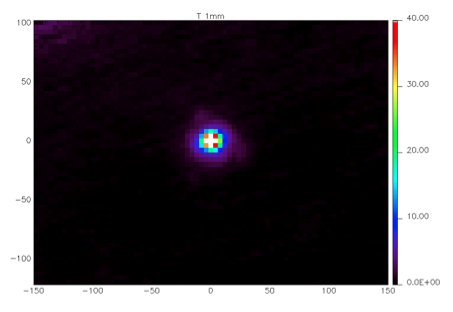
\includegraphics[scale=0.3]{figures/map_1mm_Uranus.png}
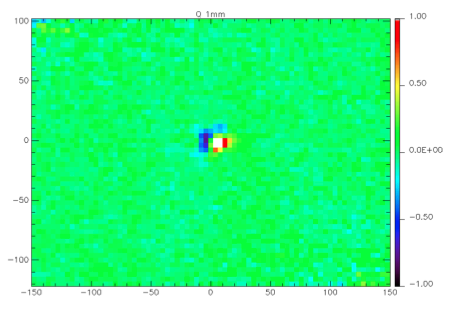
\includegraphics[scale=0.3]{figures/map_q_1mm_Uranus.png}
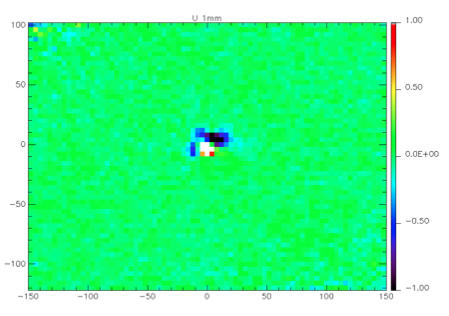
\includegraphics[scale=0.3]{figures/map_u_1mm_Uranus.png}
\caption{Intensity and polarization Q and U maps of Uranus for the 1mm channel.
 The value of the flux range is done in Jy and the x,y coordinates are in arcsec.}
\label{fig:Uranus_1mm}

  \end{figure}
\begin{figure} [t!]

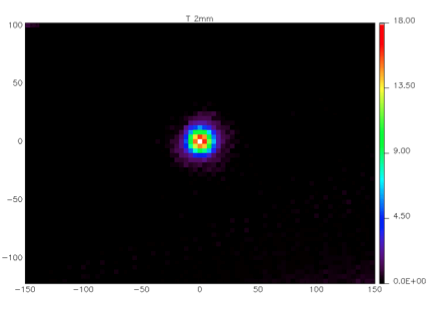
\includegraphics[scale=0.3]{figures/map_2mm_Uranus.png}
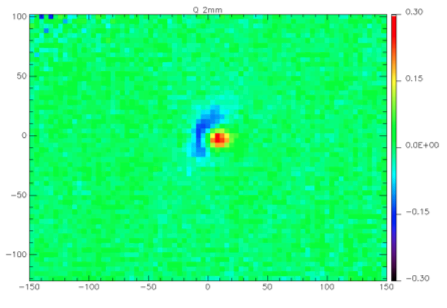
\includegraphics[scale=0.3]{figures/map_q_2mm_Uranus.png}
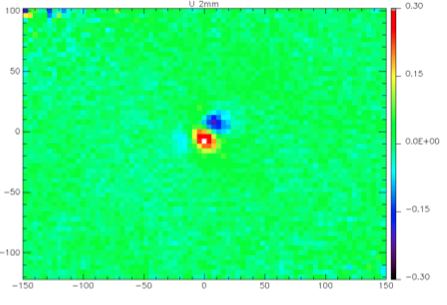
\includegraphics[scale=0.3]{figures/map_u_2mm_Uranus.png}
\caption{Intensity and polarization Q and U maps of Uranus for the 2mm channel.
 The value of the flux range is done in Jy and the x,y coordinates are in arcsec.}
\label{fig:Uranus_2mm}
  \end{figure}
\begin{figure} [t!]

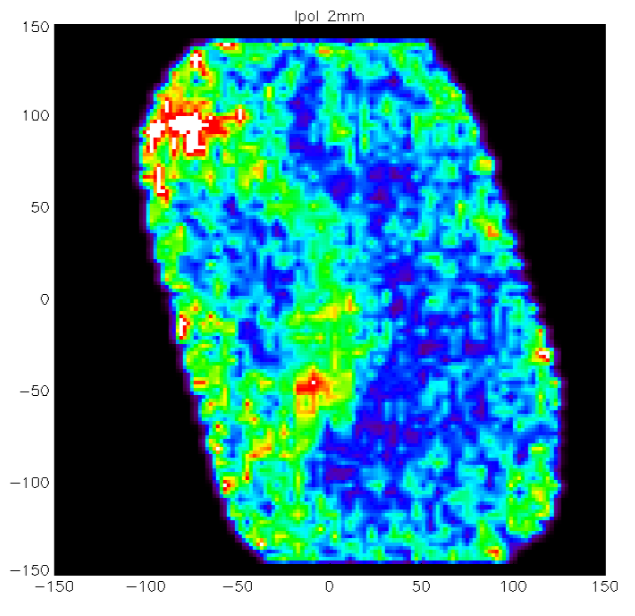
\includegraphics[width=6cm]{figures/map_casa_ipol.png}
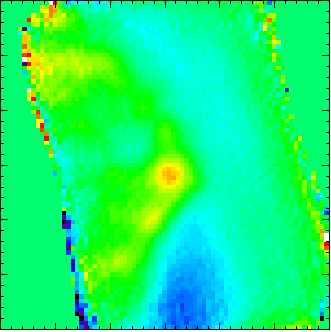
\includegraphics[width=6cm]{figures/map_2mm.png}
\caption{Polarization intensity on left and temperature intensity on right of
  Cassiopeia A for the 2 mm channel.The value of the flux range is not yet given
  because it has not been estimated with precision. The x,y coordinates are in
  arcsec.}
\label{fig:CasA_2mm}


  \end{figure}






% * I would add the Uranus map obtained in the previous run. What I have seen at the astropol2014 meeting in Grenoble looked already quite presentable.


\end{document}
